\section{Distribuições Discretas}

As distribuições discretas descrevem variáveis aleatórias que assumem valores em um
conjunto enumerável, situação comum em Computação quando o interesse recai sobre
contagens, como o número de falhas em um conjunto de requisições. Nesta seção são
apresentados os três modelos discretos mais usados, Bernoulli, binomial e Poisson,
e suas previsões teóricas são comparadas com estimativas obtidas por simulação em R.

\subsection{Conceitos fundamentais}

Uma variável aleatória $X$ é uma função $X \colon \Omega \to \mathbb{R}$ que associa
a cada resultado $\xi \in \Omega$ um número real $X(\xi)$ \cite{chan2021probability}.
Uma variável aleatória discreta assume um conjunto enumerável, finito ou infinito,
de valores, enquanto uma variável aleatória contínua assume valores em um conjunto
não enumerável \cite{harcholbalter2024probability}.

A função massa de probabilidade de uma variável aleatória discreta $X$ é definida na
Equação~\ref{eq:fmp} e atribui a cada valor possível a probabilidade de ele ser
observado. O conjunto de todos os valores possíveis de $X$ é denotado por
$X(\Omega)$.

\begin{equation}
	p_X(x) = P(X = x)
	\label{eq:fmp}
\end{equation}

\subsection{Principais distribuições discretas}

\subsubsection{Distribuição de Bernoulli}

A distribuição de Bernoulli modela um único experimento com dois resultados
possíveis, sucesso, codificado como $1$, e falha, codificado como $0$. Sua função
massa de probabilidade aparece na Equação~\ref{eq:bernoulli}, em que $0 < p < 1$ é a
probabilidade de sucesso. A esperança é $E[X] = p$ e a variância é
$\Var(X) = p(1-p)$, de modo que a variância é máxima quando $p = 0{,}5$ e se anula
nos extremos \cite{sahu2024probability}.

\begin{equation}
	p_X(0) = 1 - p, \qquad p_X(1) = p
	\label{eq:bernoulli}
\end{equation}

\subsubsection{Distribuição binomial}

A distribuição binomial descreve o número de sucessos em $n$ ensaios de Bernoulli
independentes, todos com a mesma probabilidade de sucesso $p$. Sua função massa de
probabilidade aparece na Equação~\ref{eq:binomial}, em que $\binom{n}{k}$ conta as
maneiras de escolher quais ensaios resultam em sucesso \cite{chan2021probability}. A
esperança é $E[X] = np$ e a variância é $\Var(X) = np(1-p)$.

\begin{equation}
	p_X(k) = \binom{n}{k} p^k (1 - p)^{n-k}, \qquad k = 0, 1, \ldots, n
	\label{eq:binomial}
\end{equation}

\subsubsection{Distribuição de Poisson}

A distribuição de Poisson modela o número de ocorrências de um evento em um
intervalo fixo de tempo ou espaço, quando essas ocorrências são raras e
independentes. Sua função massa de probabilidade aparece na
Equação~\ref{eq:poisson}, em que $\lambda > 0$ é a taxa média de ocorrências
\cite{chan2021probability}. Uma característica marcante é que a esperança e a
variância coincidem, $E[X] = \Var(X) = \lambda$.

\begin{equation}
	p_X(k) = \frac{\lambda^k}{k!}\, e^{-\lambda}, \qquad k = 0, 1, 2, \ldots
	\label{eq:poisson}
\end{equation}

\subsection{Modelagem de um cenário de falhas}

Para ilustrar os três modelos foi considerado um servidor cujas requisições falham
de forma independente com probabilidade $p = 0{,}05$. Cada requisição corresponde a
uma variável de Bernoulli que vale $1$ em caso de falha. O número de falhas em um
bloco de $n = 20$ requisições segue uma distribuição binomial de parâmetros $n$ e
$p$, com esperança $np = 1$. O número de falhas observadas em um intervalo de um
minuto, supondo uma taxa média de $\lambda = 2$ falhas por minuto, é modelado por
uma distribuição de Poisson.

\subsection{Simulação e resultados}

As distribuições foram simuladas com $20000$ repetições e as frequências empíricas
foram comparadas com as probabilidades teóricas. O Listing~\ref{lst:disc_gera} gera
as amostras da binomial e da Poisson.

\begin{lstlisting}[caption={Simulação das distribuições binomial e de Poisson.}, label={lst:disc_gera}]
p <- 0.05
n_req <- 20
lambda <- 2
n_rep <- 20000

falhas_binom <- rbinom(n_rep, size = n_req, prob = p)
falhas_pois  <- rpois(n_rep, lambda)
\end{lstlisting}

A Figura~\ref{fig:disc_binomial} e a Figura~\ref{fig:disc_poisson} comparam as
frequências empíricas com as probabilidades teóricas da binomial e da Poisson. Em
ambos os casos as barras empíricas praticamente coincidem com as teóricas, o que
confirma que a simulação reproduz os modelos.

\begin{figure}[H]
	\centering
	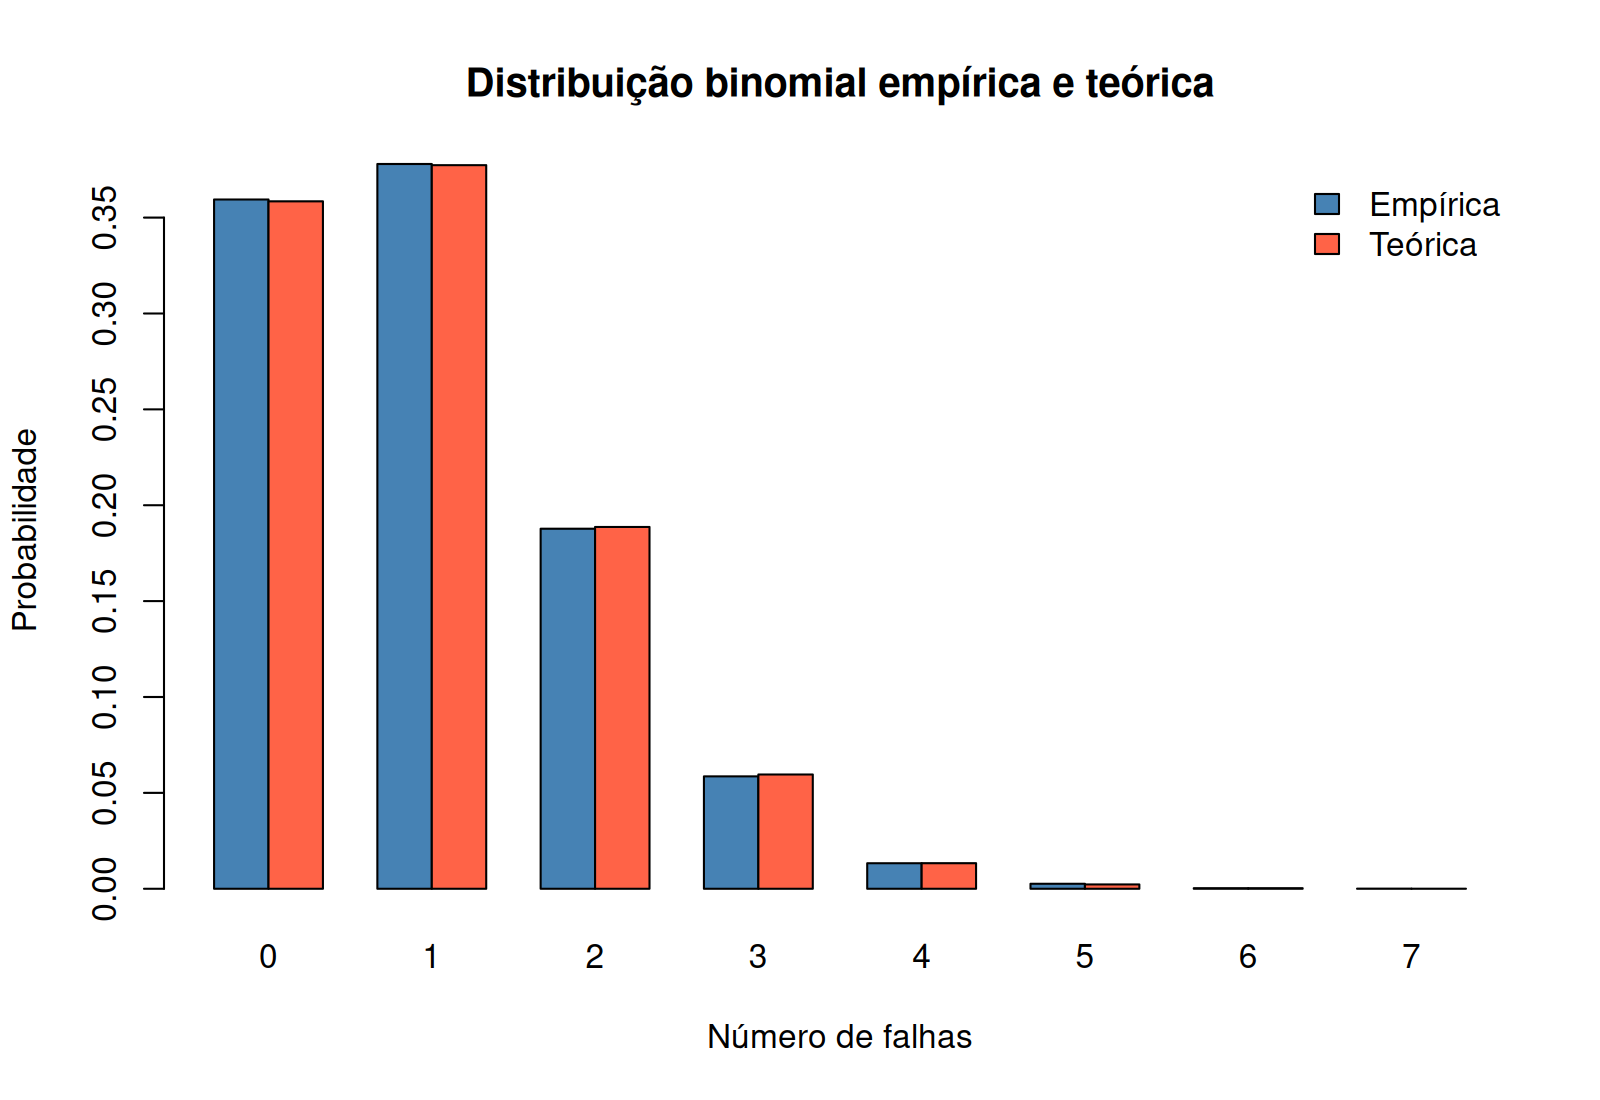
\includegraphics[width=0.8\textwidth]{secoes/03_distribuicoes_discretas/imagens/fig_binomial.png}
	\caption{Distribuição binomial empírica e teórica para $n = 20$ e $p = 0{,}05$.}
	\label{fig:disc_binomial}
\end{figure}

\begin{figure}[H]
	\centering
	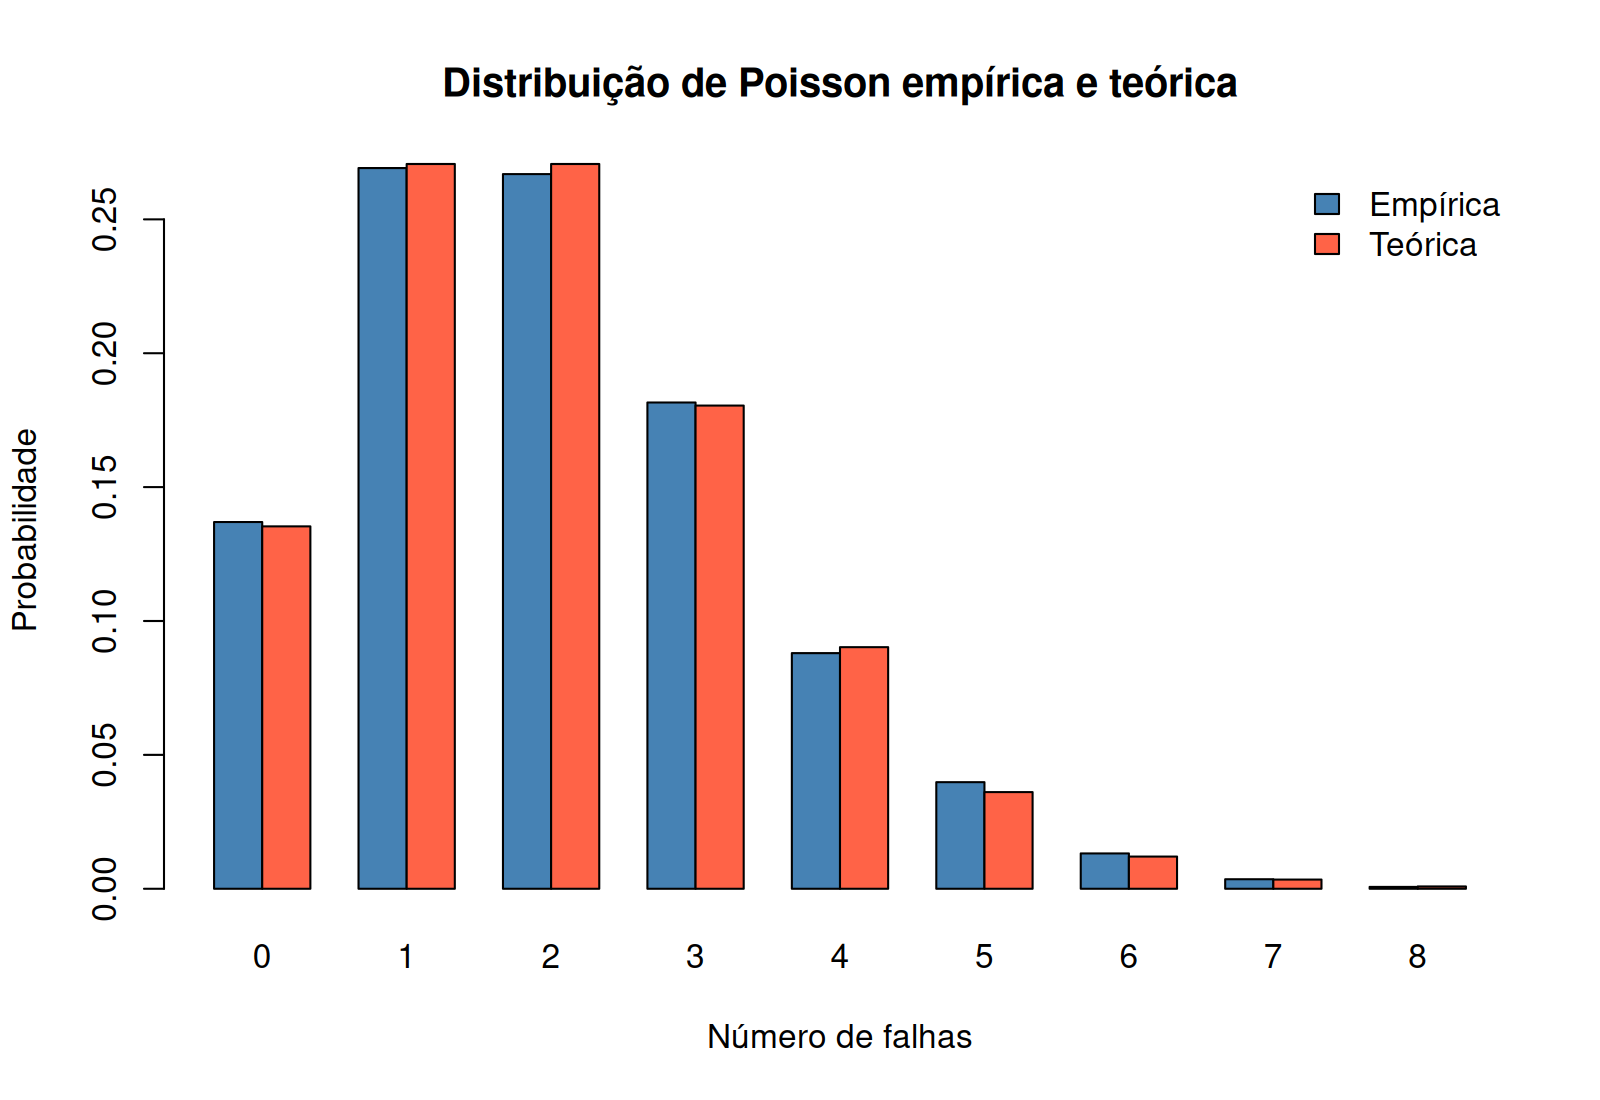
\includegraphics[width=0.8\textwidth]{secoes/03_distribuicoes_discretas/imagens/fig_poisson.png}
	\caption{Distribuição de Poisson empírica e teórica para $\lambda = 2$.}
	\label{fig:disc_poisson}
\end{figure}

A Tabela~\ref{tab:disc_medias} compara a média amostral de cada distribuição com a
esperança teórica. As diferenças aparecem apenas a partir da segunda casa decimal,
coerente com a Lei dos Grandes Números \cite{ross2010probabilidade}.

\begin{table}[H]
	\centering
	\caption{Média amostral e esperança teórica das distribuições simuladas.}
	\begin{tabular}{lcc}
		\toprule
		& Binomial $(20;\,0{,}05)$ & Poisson $(2)$ \\
		\midrule
		Empírica & 0,9976 & 2,0098 \\
		Teórica  & 1,0000 & 2,0000 \\
		\bottomrule
	\end{tabular}
	\label{tab:disc_medias}
\end{table}

A Figura~\ref{fig:disc_media} acompanha a média amostral acumulada do número de
falhas da binomial ao longo das repetições. A curva oscila bastante no início e se
estabiliza em torno do valor teórico $np = 1$ conforme o número de repetições
aumenta, o que ilustra a convergência prevista pela Lei dos Grandes Números.

\begin{figure}[H]
	\centering
	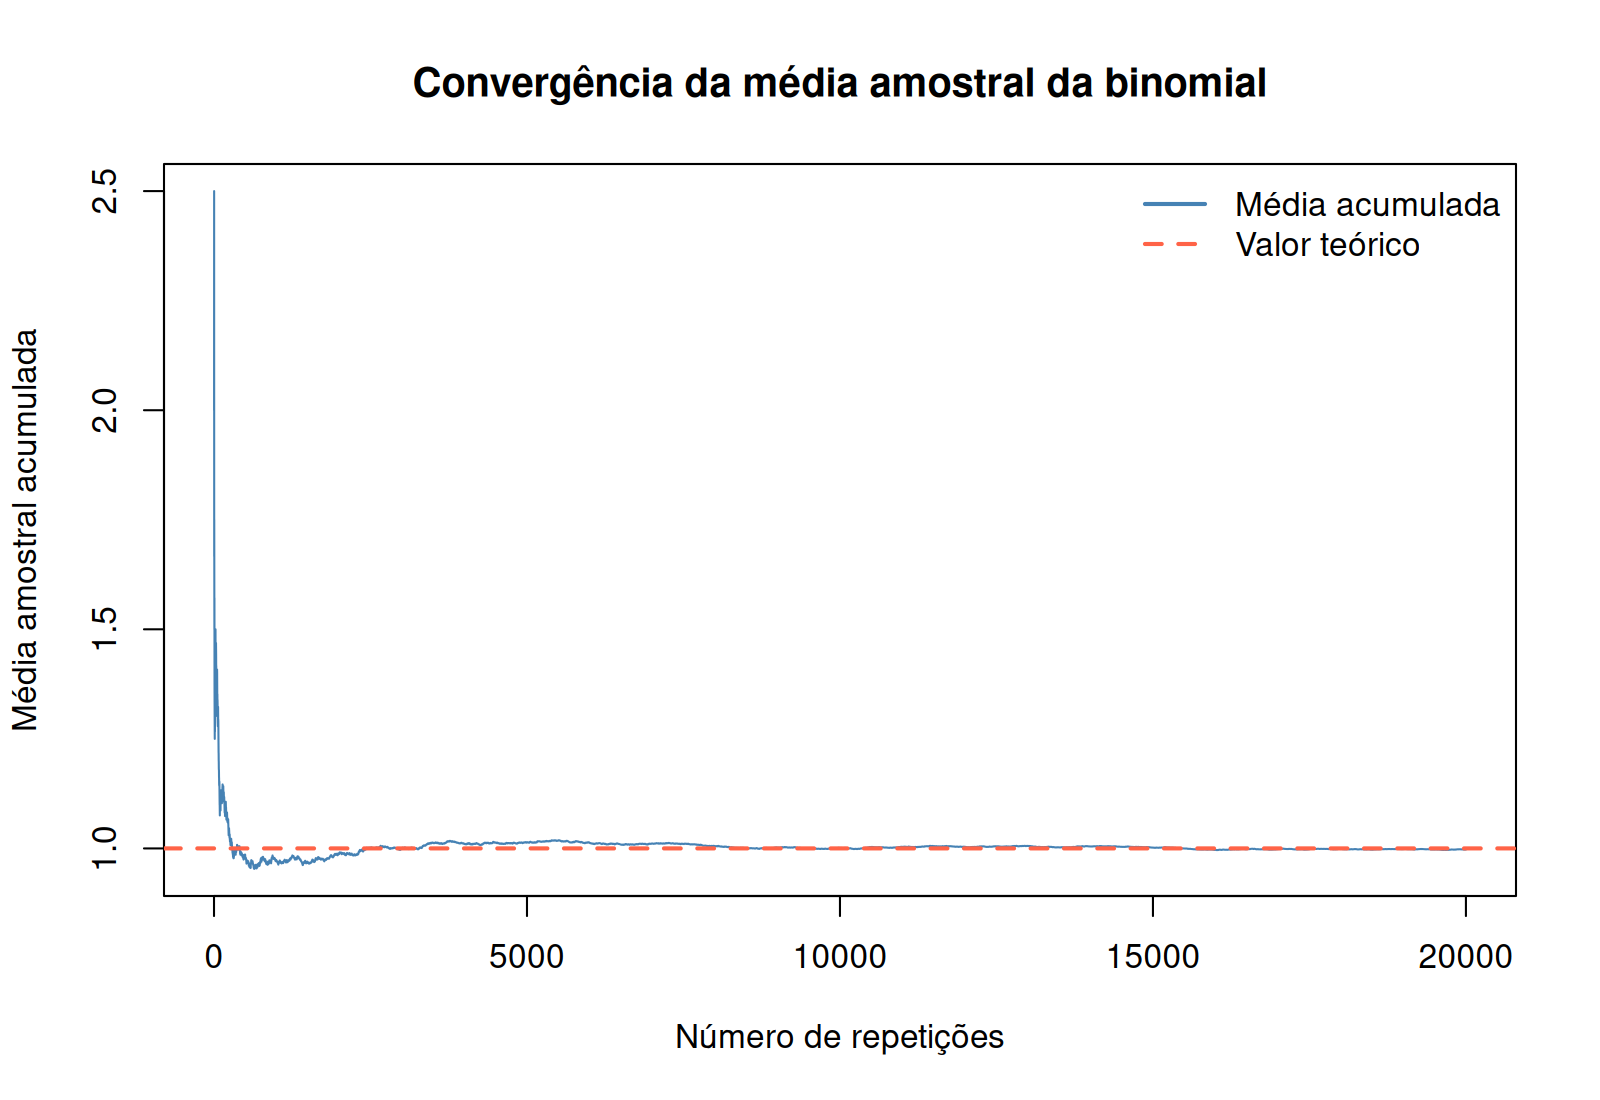
\includegraphics[width=0.8\textwidth]{secoes/03_distribuicoes_discretas/imagens/fig_media_discreta.png}
	\caption{Convergência da média amostral da binomial para a esperança $np = 1$.}
	\label{fig:disc_media}
\end{figure}
